\documentclass{article} % There are various classes of documents, we will see a few later

\usepackage{booktabs}
\usepackage{graphicx}
\usepackage{tikz}
\usepackage{amsmath}

\title{Choose a title}
\author{Sachchidanand Kumar}
\date{\today}

\begin{document} % This line starts the document

\begin{abstract}
    This document contains some basic \LaTeX~code that will be useful to me in the future 
\end{abstract}

\maketitle

Hello, World!\\
Here is how to use `Single quotes` and here is how to use  ``Double quotes``.

\begin{itemize}
    \item Unordered item number 1
    \item Unordered item number 2
    \item Unordered item number 3
\end{itemize}

\begin{enumerate}
    \item Ordered item number 1
    \item Ordered item number 2
    \item Ordered item number 3
\end{enumerate}

\begin{tabular}{|l|c|r|}
     \hline
     Name  &  Gender  & Start Time \\
     \hline
     Sachchidanand  &  Male  &  1100\\
     \hline
     Manoj  &  Male  &  1200\\
     \hline
     Unnati  & Female  &  1500\\
     \hline
\end{tabular}

\begin{tabular}{l|c|r}
     \\
     \toprule
     Name & Gender & Start Time\\
     \midrule
     Sachchidanand & Male & 1100\\
     Unnati & Female & 1500\\
     Manoj & Male & 1200\\
     \bottomrule
\end{tabular}

\begin{center}
    \includegraphics[width=.6\textwidth]{ange.jpg}
\end{center}

\begin{center}
    
\begin{tikzpicture}
        \draw [ultra thick, color = blue] (0,0) -- (0,2);
        \draw [ultra thick, color = blue] (0,0) -- (2,0);
        \draw [ultra thick, color = blue] (0,2) -- (2,2);
        \draw [ultra thick, color = blue] (2,0) -- (2,2);
    \end{tikzpicture}
\end{center}

\begin{center}
    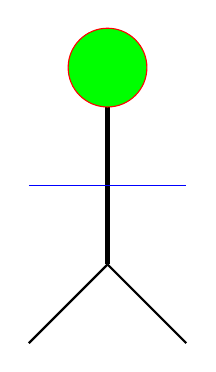
\begin{tikzpicture}
        \draw [ultra thick] (0, 0) -- (0, 2);
        \draw [thin, color = blue] (-1,1) -- (1,1);
        \draw [thick] (0,0) -- (1,-1);
        \draw [thick] (0,0) -- (-1,-1);
        \draw [color = red, fill = green] (0,2.5) circle (0.5);
    \end{tikzpicture}
\end{center}

Figure~\ref{my_picture} show my picture.

\begin{figure}[!htbp]
    \begin{center}
        \includegraphics{ange.jpg}
    \end{center}
    \caption{Sachchidanand Kumar}
    \label{my_picture}
\end{figure}

Table~\ref{my_table} my data

\begin{table}[!hbtp]
    \begin{center}
        \begin{tabular}{l|c|r}
            \toprule
            Name & Gender & pointer
            \midrule
            Sachchidanand Kumar & Male & 9.82\\
            \bottomrule
        \end{tabular}
    \end{center}
    
    \caption{My Data}
    \label{my_table}
\end{table}

\section{My first section} \lable{first_section}

This is a section with a few subsections.

    \subsection{A part of my first section}
    
    Here I could write about the problem I'm trying to solve.
    
    \subsection{Another part of my first section}
    
    In this section I could solve the problem.
    
        \subsubsection{Further fragmentation ...... }
        
\section{ My second section }\lable{second_section}

In Section \ref{first_section} We saw that ... 

Mathematics can be typed into \LaTeX\ as $x^2$ and/or \((a+b)^2=a^2+2ab+b^2\). 

\[
    \int_{0}^{5}x^2dx
\]

\[
    \sum_{i=1}^{n}i=\frac{n(n+1)}{2}
\]

\begin{equation}\lable{my_first_equation}
    e=mc^2
\end{equation}

In equation (\ref{my_first_equation}) we have a very well known relationship.

\[
    x^2 = \text{ implies } x = \pm 1
\]

\begin{enumerate}
    \item \(a+b\)
    \item \(a-b\)
    \item \(-a\)
    \item \(ab\)
    \item \(a\cdot b\)
    \item \(a\times b\)
    \item \(a/b\)
    \item \({a \over b}\)
    \item \(\frac{a}{b}\)
\end{enumerate}

\[
    \begin{pmatrix}
        a&b\\
        c&d\\
        e&f\\
        
    \end{pmatrix}
\]

\[
    \begin{vmatrix}
        a&b\\
        c&d\\
        e&f\\
        
    \end{vmatrix}
\]

\[
    \begin{matrix}
        a&b\\
        c&d\\
        e&f\\
        
    \end{matrix}
\]



\end{document}